\subsection{Apparatus for Manufacturing of Polymer Matrix Composites}
A set DA 409U/G35 150 prepeg sheets were provided for the purposes of designing and forming both the $0\degree$ and $45\degree$ specimens.  A sharp utility knife was provided to slice the sheets into the proper dimensions.  Due to the high sensitivity to local humidity and temperature, the manufacturing process was done in a large, well ventilated room with an analog hygrometer/digital thermometer.  The analog hygrometer had a relative humidity accuracy of 2.5\% and resolution of 1.0\%; the digital thermometer had an accuracy of $1.5\degree$F and resolution of $0.1\degree$F.  For the purpose of weighing the specimen prior to cure, an electronic top loading balance scale was provided with a linearity of $\pm 0.001$ grams and $4.0$ second stabilization time.  During the measuring, cutting, and assembling of the specimen, slightly unconventional methods of chilling the composite were used to rapidly decrease the local temperature of the material to prevent premature curing and mitigate the slow increase of void content in the composite matrix.  Some methods included compressed air cans or thermal cold-sinks.  Additional information about the tools used in experiment six may be found in Table \ref{tab:equipmentpart1} below and labelled pictures displaying the components may be found in Figure \ref{fig:exp1}.

The lay-up portion of the lab primarily focused on setting the laminate within layers peel ply, bleeder ply, and release films.  Each of these layers served a purpose of absorbing, displacing, and stabilizing the resin during the thermosetting process.  The components used during the lay-up process are provided in Table \ref{tab:equipmentpart1} (\textit{continued}) and the pictures displayed in Figure \ref{fig:exp1b}.  Images were provided by the lab manual \cite{labmanual}, and included the key components for experiment 1.

\begin{table}[h!]
    \centering
    \caption{Equipment and Specifications for Specimen Manufacturing}
    \begin{tabular}{|c|C{0.25\textwidth}|C{0.25\textwidth}|C{0.12\textwidth}|C{0.2\textwidth}|}\toprule
        \textbf{No.} & \textbf{Item} & \textbf{Description} & \textbf{Accuracy} & \textbf{Use in Experiment} \\ \midrule
        \textbf{1} & DA 409U/G35\newline 150 prepreg & Unidirectional reinforcement,\newline G35 graphite fibers,\newline 409 epoxy matrix, Prepreg planar density of $\rho = 150 g/m^2$ & N/A & Slices were cut out of preform sheets to construct polymer composite specimen \\ \hline
        \textbf{2} & Traceable\textsuperscript{\tiny\textregistered} Analog Hygrometer/ \newline Digital Thermometer & 5.0 inch dial,\newline RH range: 0\% - 100\%.\newline Thermometer range: $23.0\degree-131.0\degree$F & RH $2.5\%$, T $1.5\degree$F & Placed in layup, weighing, and hot press rooms. \\\hline
        \textbf{3} & Electronic Top Loading Balance & Highly sensitive scale & $\pm0.001$ g & Weigh composite specimen \& bleeder cloth before and after cure \\\hline
        \textbf{4} & Carver Programmable Hot press & Electrical Platens,\newline Max Temperature $850\degree$F,\newline Max Pressure 24 tons & N/A & Hot press to thermoset the composite \\\hline
    \end{tabular}
    \label{tab:equipmentpart1}
\end{table}

\begin{table}[h!]
    \centering
    \begin{tabular}{|c|C{0.25\textwidth}|C{0.25\textwidth}|C{0.12\textwidth}|C{0.2\textwidth}|}
        \multicolumn{5}{c}{\textbf{Table 1} (\textit{continued})\textbf{:} \textbf{Lay-up Materials}} \\\midrule
        \textbf{5} & AirTech N10 Bleeder Cloth & Absorb excess resin \& \newline Provide vacuum path to remove volatiles & N/A & Bleeder cloth to absorb resin \\\hline
        \textbf{6} & Release-Ease 234 TFP Peel Ply & Teflon coated to prevent resin sticking & N/A & Porosity allowed uniform displacement of resin while preventing undesired adhesion \\\hline
        \textbf{7} & A4000R Non-perforated TFP Film & Placed between press and layup materials & N/A & Prevents lay-up materials from adhering to the mold and tool \\\hline
        \textbf{8} & 2024-T3 Aluminium Mold & Three $1.0 x 7.0$ slots for lay-up material & N/A & Holds the lay-up material while placed in hot press \\\bottomrule
    \end{tabular}
\end{table}

\begin{figure}[!h]
  \begin{subfigure}[t]{.4\textwidth}
    \centering
    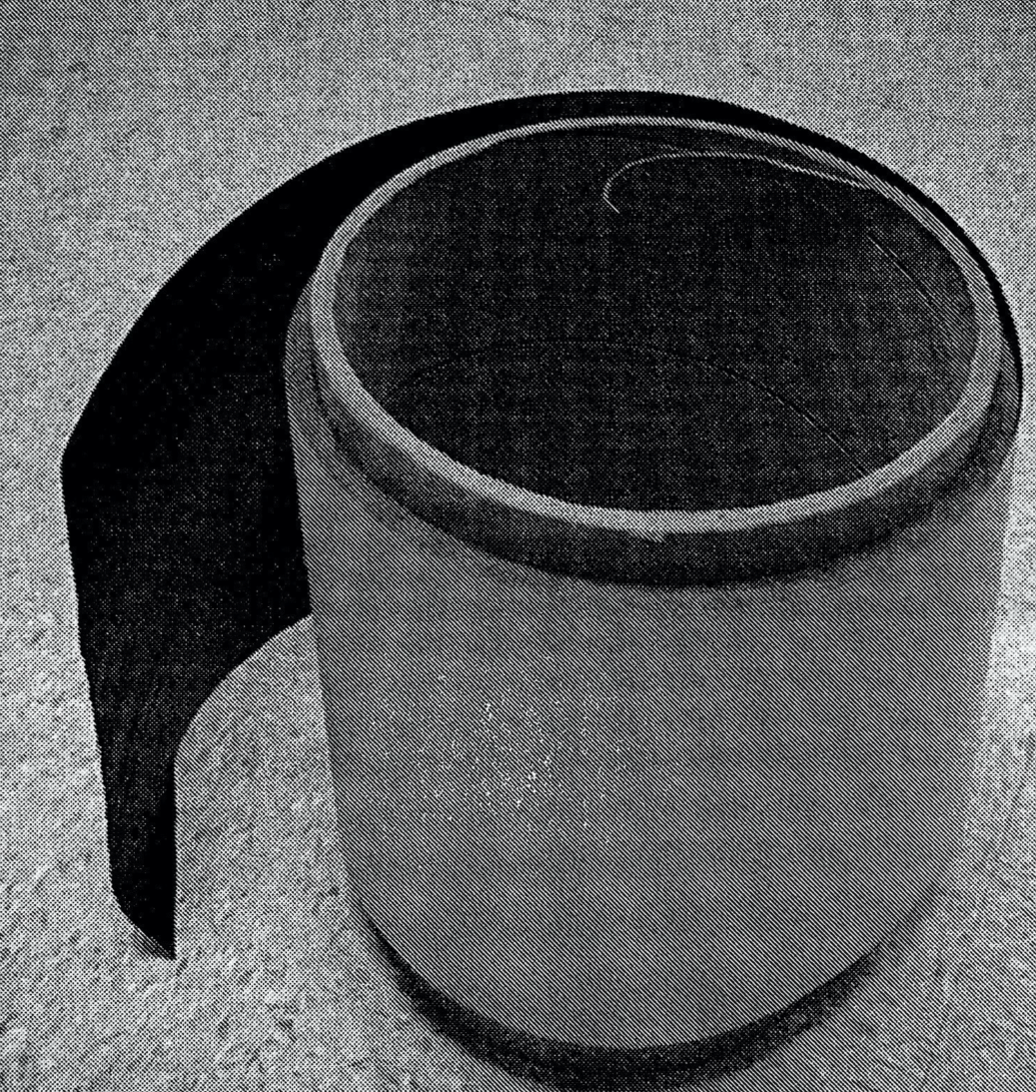
\includegraphics[width=\linewidth]{Pictures/Apparatus/Experiment 1/one.png}
    \caption{\textbf{1.} DA 409U/G35 150 prepreg}
  \end{subfigure}
  \hfill
  \begin{subfigure}[t]{.4\textwidth}
    \centering
    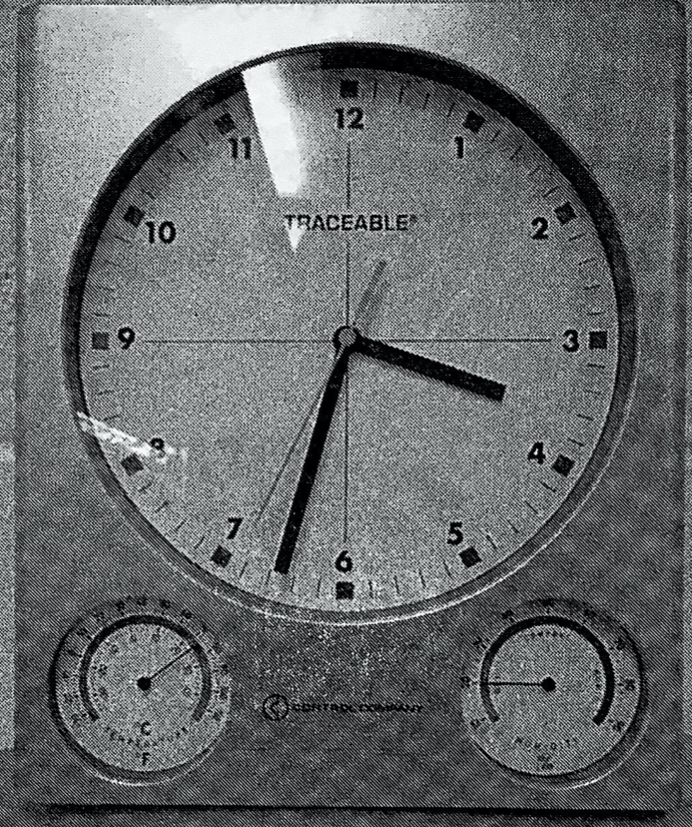
\includegraphics[width=\linewidth]{Pictures/Apparatus/Experiment 1/two.png}
    \caption{\textbf{2.} Analog Hygrometer/Digital Thermometer}
  \end{subfigure}

  \medskip

  \begin{subfigure}[t]{.4\textwidth}
    \centering
    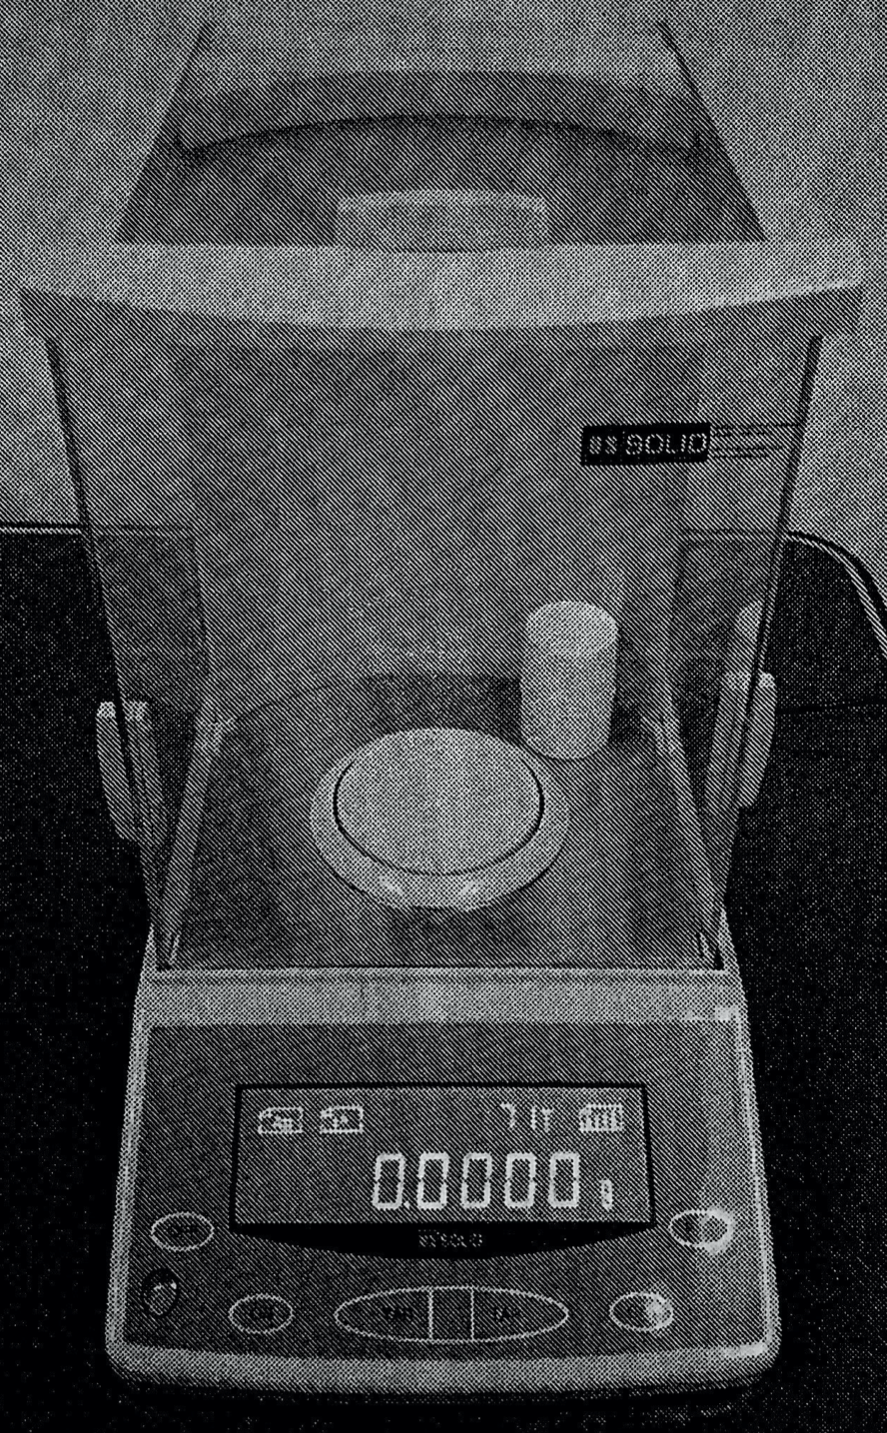
\includegraphics[width=\linewidth]{Pictures/Apparatus/Experiment 1/three.png}
    \caption{\textbf{3.} Electronic Top Loading Balance}
  \end{subfigure}
  \hfill
  \begin{subfigure}[t]{.4\textwidth}
    \centering
    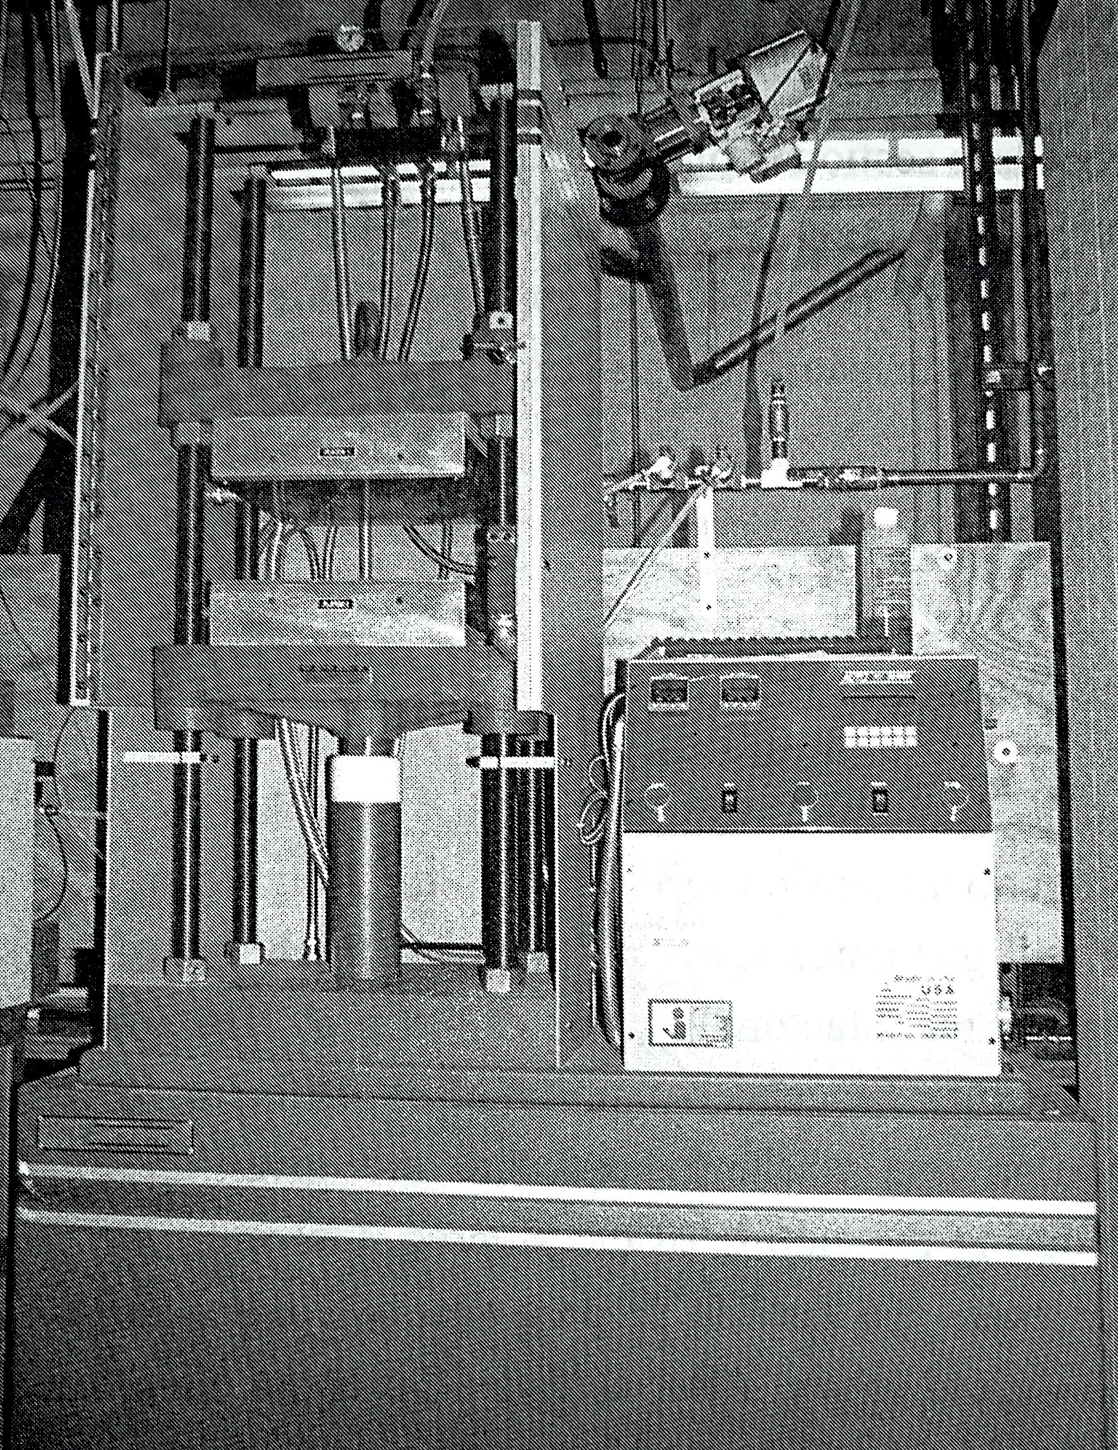
\includegraphics[width=\linewidth]{Pictures/Apparatus/Experiment 1/eight.png}
    \caption{\textbf{4.} Carver Programmable Hot Press}
  \end{subfigure}
  \caption{Experiment 1 Assembly Tools}
  \label{fig:exp1}
\end{figure}

\clearpage

\begin{figure}[!h]
  \begin{subfigure}[t]{.4\textwidth}
    \centering
    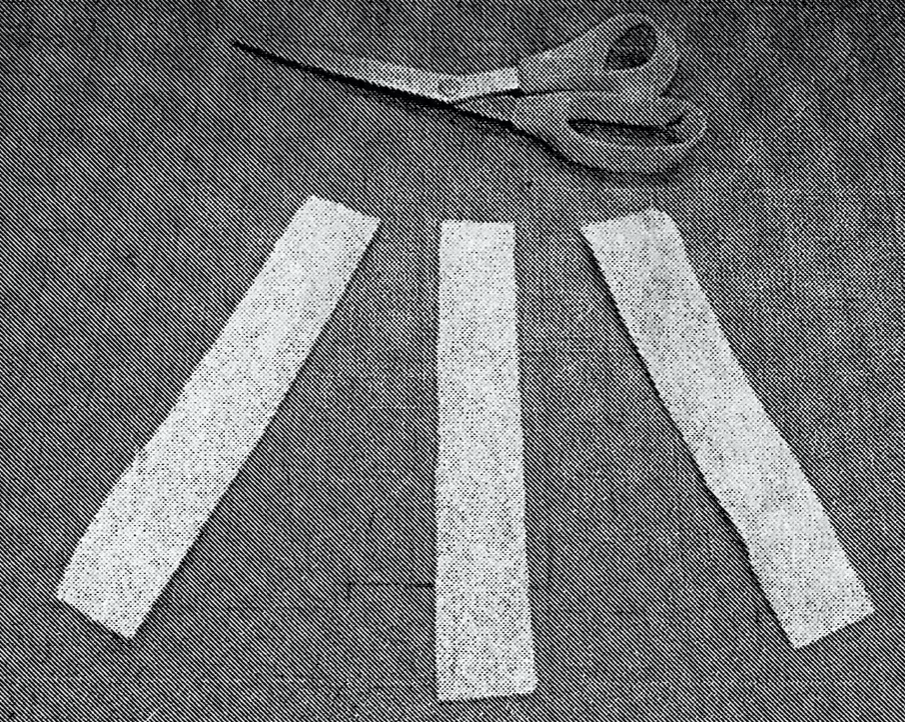
\includegraphics[width=\linewidth]{Pictures/Apparatus/Experiment 1/four.png}
    \caption{\textbf{5.} AirTech N10 Bleeder Cloth}
  \end{subfigure}
  \hfill
  \begin{subfigure}[t]{.4\textwidth}
    \centering
    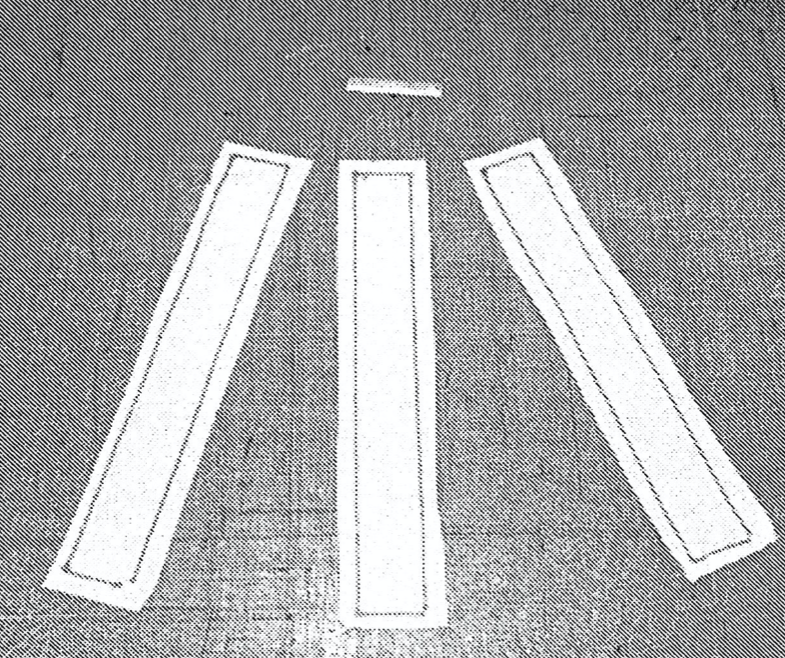
\includegraphics[width=\linewidth]{Pictures/Apparatus/Experiment 1/five.png}
    \caption{\textbf{6.} Release-Ease 234 TFP Peel Ply}
  \end{subfigure}

  \medskip

  \begin{subfigure}[t]{.4\textwidth}
    \centering
    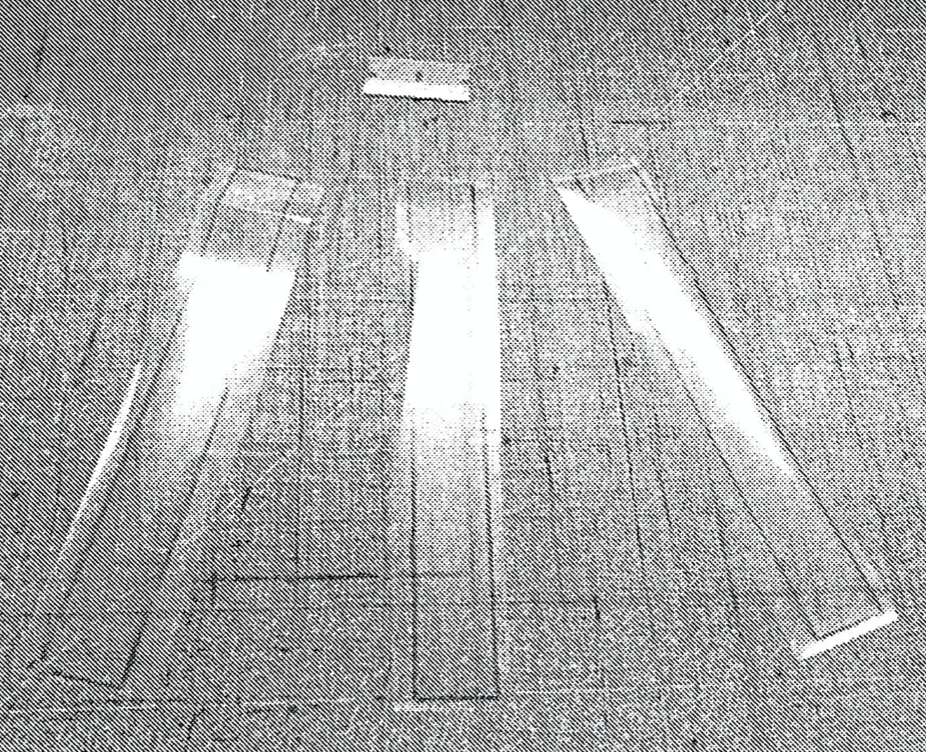
\includegraphics[width=\linewidth]{Pictures/Apparatus/Experiment 1/six.png}
    \caption{\textbf{7.} A4000R Non-perforated TFP Film}
  \end{subfigure}
  \hfill
  \begin{subfigure}[t]{.4\textwidth}
    \centering
    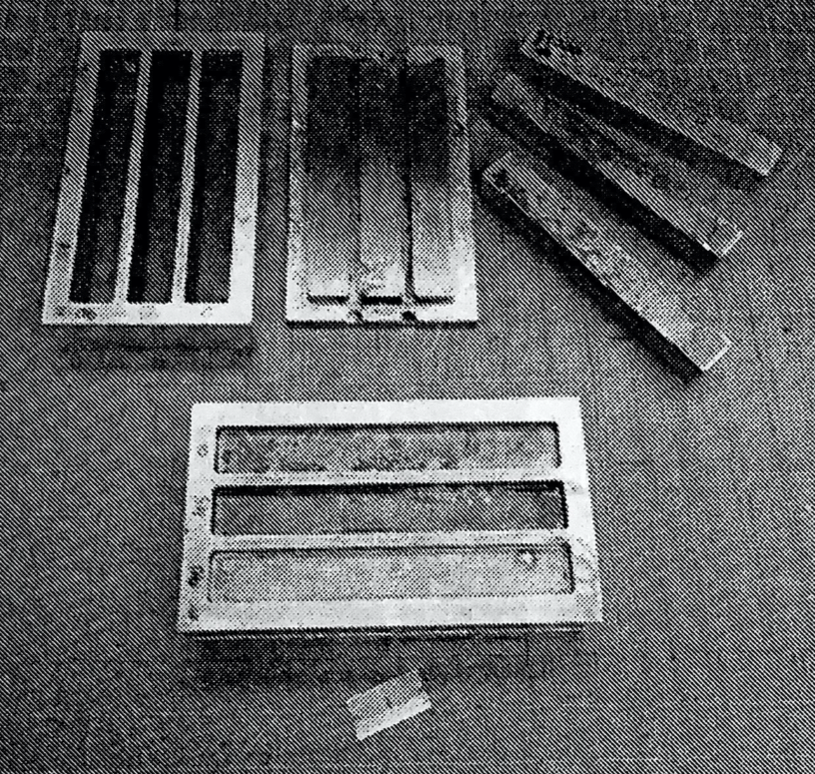
\includegraphics[width=\linewidth]{Pictures/Apparatus/Experiment 1/seven.png}
    \caption{\textbf{8.} 2024-T3 Aluminium Mold}
  \end{subfigure}
  \caption{Experiment 1 Lay-up Tools}
  \label{fig:exp1b}
\end{figure}

\vspace{-0.5in}
\subsection{Apparatus for Mechanical Property Testing of Composite Materials}
Experiment 6 focused on testing the composite specimen created in experiment 1.  To determine the mechanical properties of the composite materials, the specimen were loaded with tension using the Instron model 4483, screw-driven machine.  The Instron 4483 has a load cell to measure the force exerted on the specimen.  In addition, the strain was measured using the Instron 2630-100 static extensometer, which observes the strain of the specimen with an electrical calibration accuracy (ECA) of approximately $\pm0.06$ full range output (FRO).  The two devices, connected to a laboratory computer to record data, were used to test the three specimen.
\newpage
Additional information about the apparatus used in experiment six may be found in Table \ref{tab:equipmentpart3} below and labelled pictures displaying the components may be found in Figure \ref{fig:exp6setup}.

\begin{table}[h!]
    \centering
    \caption{Equipment and Specifications for Uniaxial Tension Testing}
    \begin{tabular}{|c|C{0.25\textwidth}|C{0.25\textwidth}|C{0.12\textwidth}|C{0.2\textwidth}|}\toprule
        \textbf{No.} & \textbf{Item} & \textbf{Description} & \textbf{Accuracy} & \textbf{Use in Experiment} \\ \midrule
        \textbf{1} & Instron model 4483 & Screw-driven tension compression tests\newline Max load 20 kips & N/A & Used to exert tension load on specimen \\\hline
        \textbf{2} & Instron model 2630-100 static Extensometer & 1.0 inch gauge length & ECA:\newline $\pm0.06$ FRO \cite{extensometer} & Measure specimen strain \\\hline
    \end{tabular}
    \label{tab:equipmentpart3}
\end{table}

\begin{figure}[!h]
    \centering
    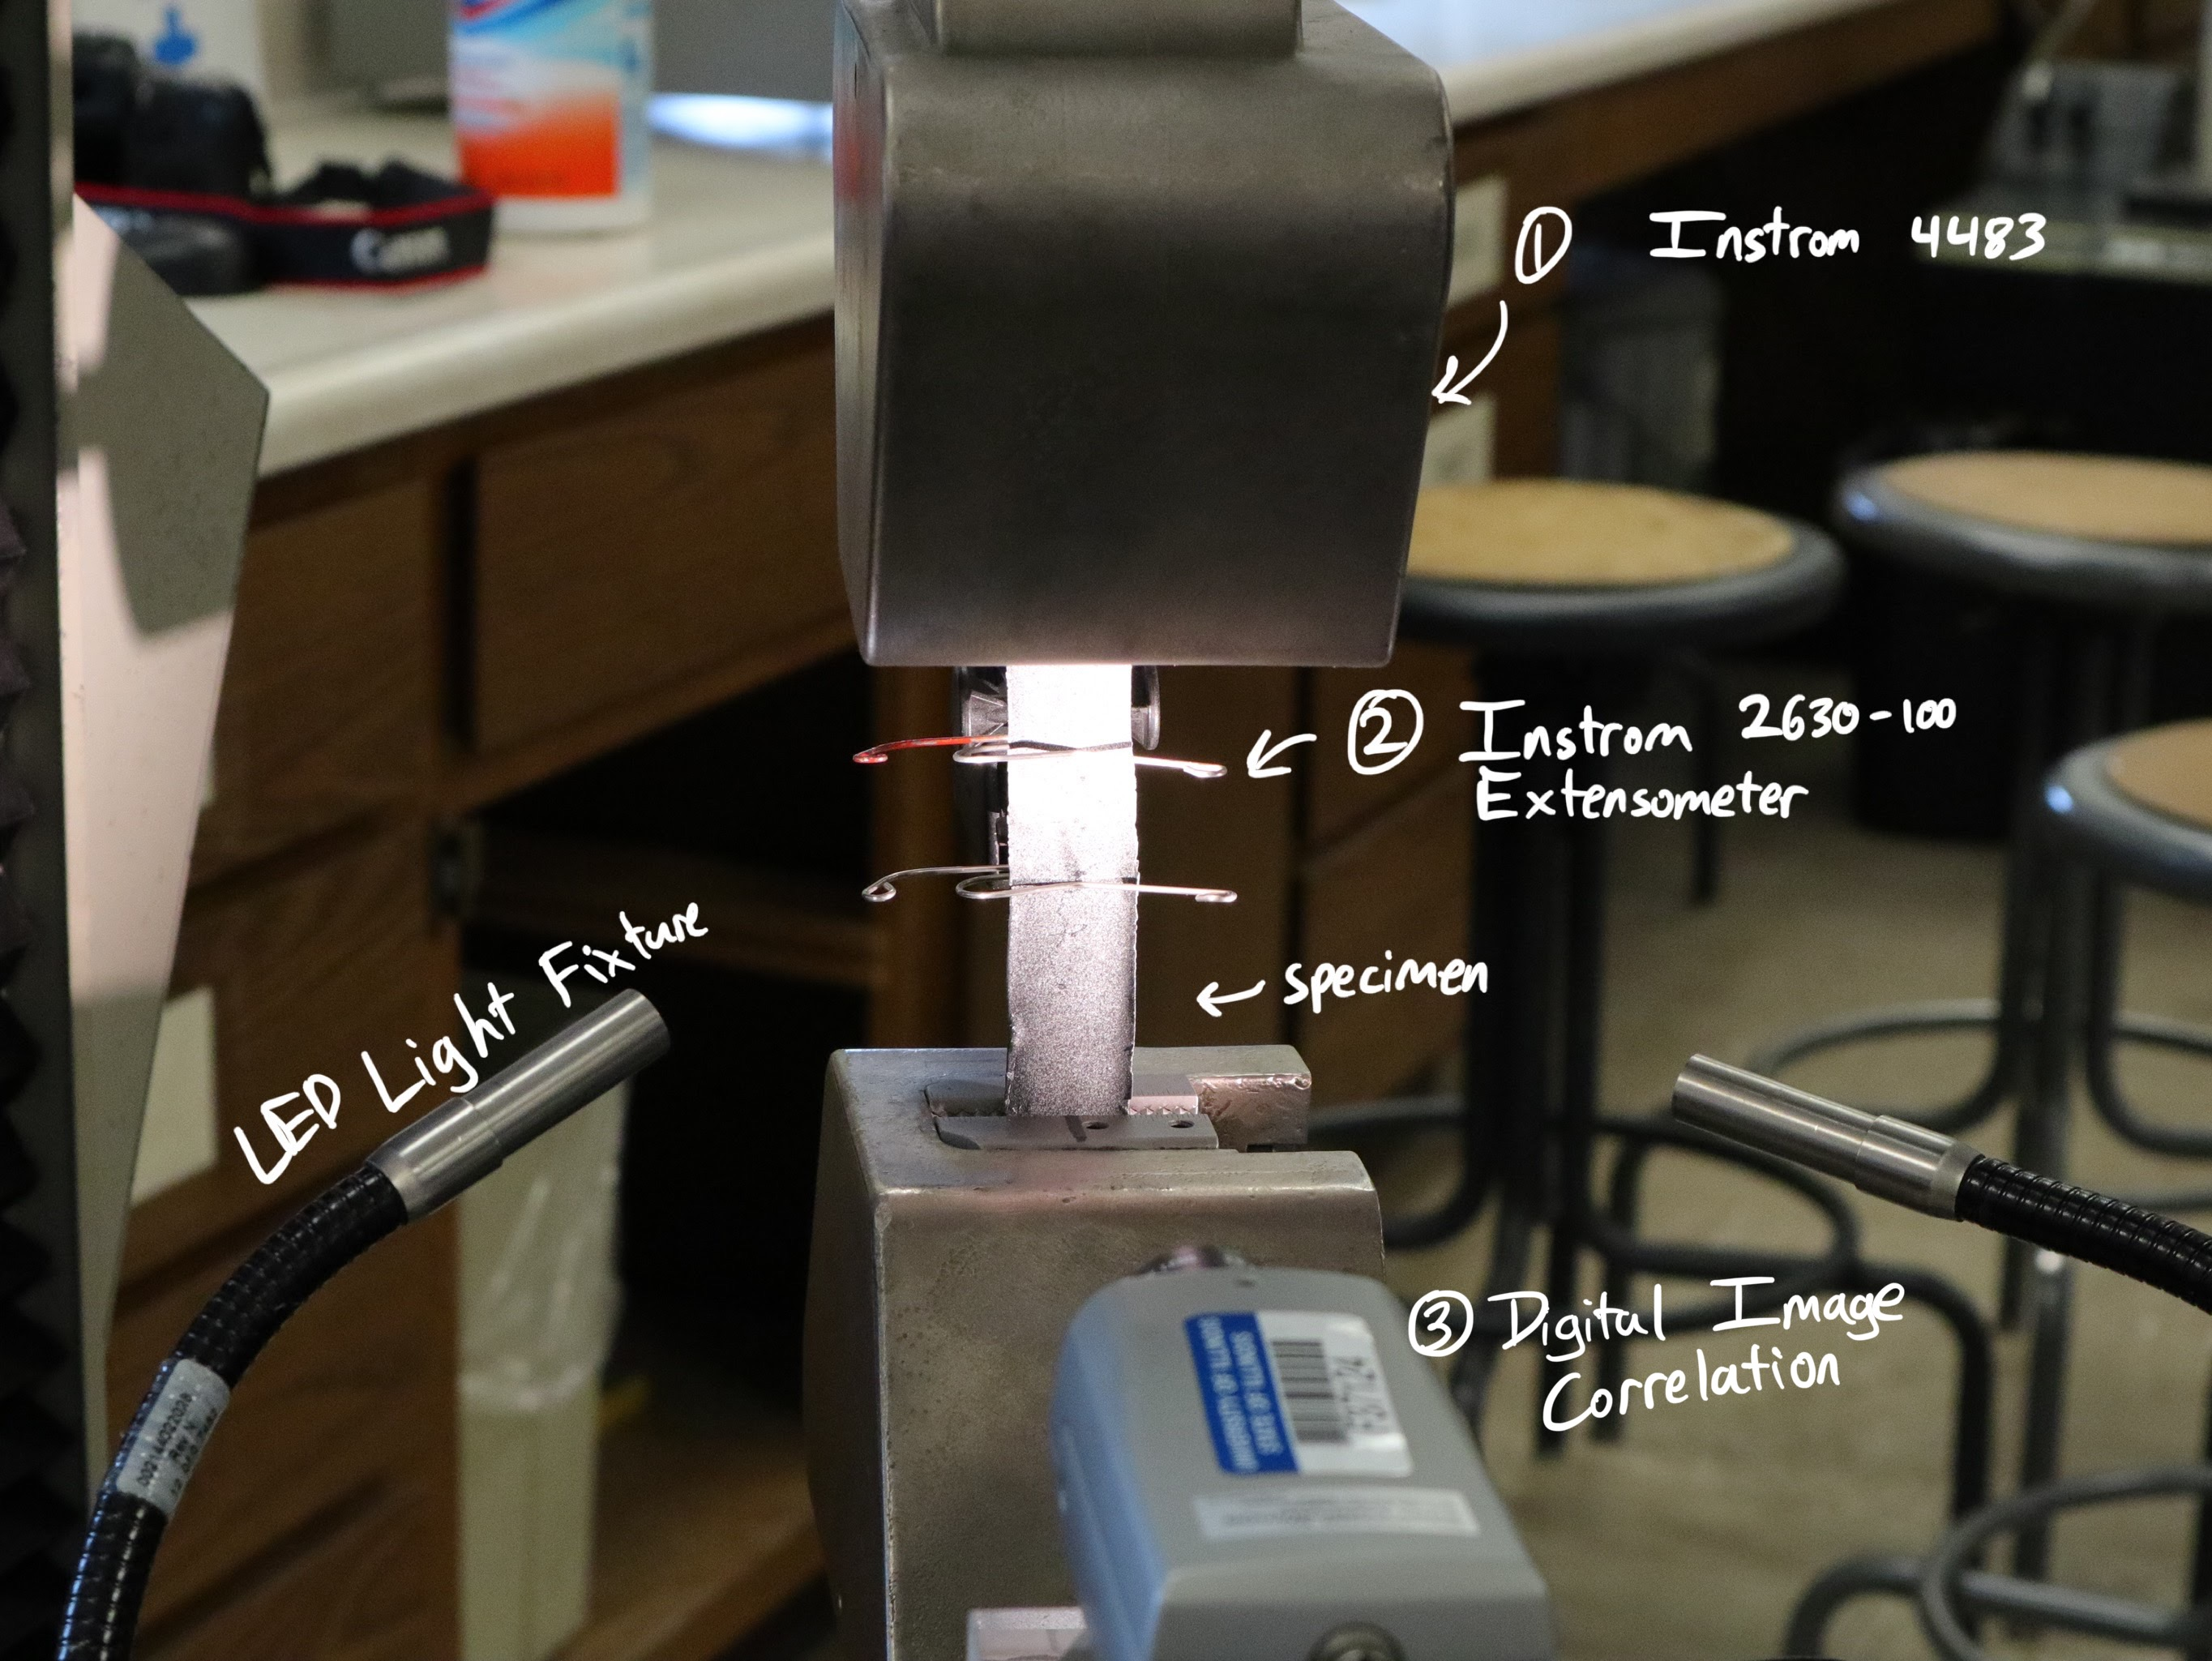
\includegraphics[width=0.95\textwidth]{Pictures/Apparatus/Experiment 6/testsetup_extensometer.JPG}
    \caption{Annotated Testing Setup}
    \label{fig:exp6setup}
\end{figure}